\documentclass[tikz,border=10pt,fleqn]{article}
\title{Bell's spaceship paradox}
\author{Hans Halvorson}
\date{\today}
\usepackage{pgfplots}
\pgfplotsset{compat=newest}

%% to do: bibliography
\usepackage{doi}
\usepackage[backend=biber,natbib=true,style=authoryear]{biblatex}
\addbibresource{str.bib}

\usepackage{amsfonts}
\usepackage{amsthm}
\theoremstyle{definition}
\usepackage{amsthm}
\newtheorem*{question}{Question}
\newtheorem*{fact}{Fact}

\newcommand{\vecc}[1]{\overrightarrow{#1}}

\begin{document}

%% don't bury the lede: "the string" is ambiguous!

\maketitle

TO DO:
\begin{itemize}
\item Is it correct that Bob's coordinatization of Alice's motion will
  be in the Rindler coordinates?
\item What is Alice's velocity relative to Bob?   
\end{itemize}

\section{Introduction}

In his famous article ``How to teach special relativity'', John Bell
\citeyearpar{bell} claims that a certain physical event $E$ occurs in
a certain scenario. He then goes on to argue that the occurence of
this event has some rather interesting implications for the
interpretation of special relativity. Over the past few decades,
several philosophers have cited Bell's article, often in support of
the claim that special relativity is, strictly speaking, false, or at
least incomplete, i.e.\ just a principle theory in wait of a
constructive underpinning \citep[see][]{brown1999,brown2004}.

Here is Bell's description of the relevant scenario.
\begin{quote} Three small spaceships, A, B, and C, drift freely in a
  region of space remote from other matter, without rotation and
  without relative motion, with B and C equidistant from A (Fig. 1).
  On reception of a signal from A the motors of B and C are ignited
  and they accelerate gently (Fig. 2).  Let ships B and C be
  identical, and have identical acceleration programmes. Then (as
  reckoned by an observer in A) they will have at every moment the
  same velocity, and so remain displaced one from the other by a fixed
  distance. Suppose that a fragile thread is tied initially between
  projections from B and C (Fig. 3). If it is just long enough to span
  the required distance initially, then as the rockets speed up, it
  will become too short, because of its need to Fitzgerald contract,
  and must finally break. \end{quote} It seems that most people agree
with Bell's claim that the thread will break in this scenario ---
despite disagreeing about what it means for special relativity. My
primary claim is that, in this scenario, there is no physical object
that could be called ``the thread''. Indeed, in special relativity, no
extended physical object can undergo constant acceleration.

\section{Preliminaries}

We assume that Alice (leading) and Bob (trailing) receive the
instruction to accelerate at the same time (in what was originally
their common reference frame). Bob's trajectory (blue) is given by
\[ b(t) \: = \: (\sinh(t),\cosh(t) ) , \]
in the coordinates of the laboratory frame. Here we use the coordinate
convention $(\mathsf{time},\mathsf{space})$. Similarly, Alice's trajectory
(green) is given by
\[ a(t) \: = \: (\sinh (t),\cosh (t)+1) .\] Since $b(t)=(0,1)+a(t)$,
we have $b'(t)=a'(t)$, where \[ a'(t) \: = \: (\sinh (t),\cosh(t)) ,\]
and
\[ a''(t) \: = \: (\cosh (t),\sinh (t)) .\] In particular,
\[ \| a''(t) \|^2 = \sinh ^2 (t)-\cosh ^2(t) = 1 ,\] for all $t$,
i.e.\ the magnitude of Alice and Bob's accelerations are
constant. Similarly, the magnitude of Alice and Bob's proper
velocities are constant. In contrast, Alice's velocity in the
laboratory frame is $v(s)=\sinh (s)/\cosh (s)$ which is zero at $s=0$
while $\lim _{s\to\infty }v(s)=1$.

In the following diagram, the red vector is tangent to Bob's
trajectory at the point $(\sqrt{2},1)$. The dashed blue line is Bob's
orthogonal spacelike hypersurface when he is located at
$(\sqrt{2},1)$, and the dashed green line is Alice's orthogonal
spacelike hypersurface when she is located at $(\sqrt{2}+1,1)$.

\bigskip \noindent 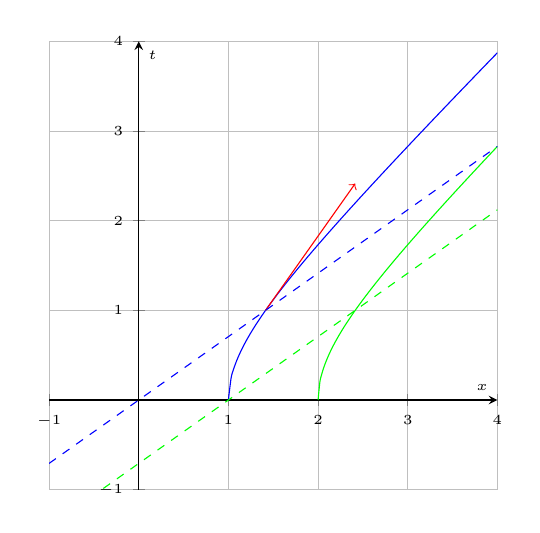
\begin{tikzpicture}
    \begin{axis}[
        axis lines=middle,
        xlabel={$x$},
        ylabel={$t$},
        xlabel style={font=\tiny}, % Makes the x-axis label smaller
        ylabel style={font=\tiny}, 
        xmin=-1, xmax=4,
        ymin=-1, ymax=4,
        grid=both,
        grid style={line width=.1pt, draw=gray!10},
        major grid style={line width=.2pt,draw=gray!50},
        axis equal image,
        legend pos=north west,
        tick label style={font=\tiny}, 
    ]
    % Original hyperbola (positive y values only)
    \addplot[domain=1:4, samples=100, smooth, blue] {sqrt(x^2 - 1)};

    % Shifted hyperbola (positive y values only)
    \addplot[domain=2:4, samples=100, smooth, green] {sqrt((x-1)^2 - 1)};

    % Tangent vector at x=2
    \draw[->, red] (axis cs:{sqrt(2)},1)--++(axis direction cs:1,{sqrt(2)});

    % Calculate slope
    \pgfmathsetmacro{\slope}{1/sqrt(2)}

    % Calculate y-intercept
    \pgfmathsetmacro{\yintercept}{1 - \slope*sqrt(2)}

    % Plot the line
    \draw[blue, dashed] (-1,{\slope*-1 + \yintercept}) -- (4,{\slope*4 + \yintercept}) node[right] {};

    \pgfmathsetmacro{\yinterceptNew}{1 - \slope*(1 + sqrt(2))}

    % Plot the new line
    \draw[green, dashed] (-1,{\slope*-1 + \yinterceptNew}) -- (4,{\slope*4 + \yinterceptNew}) node[right] { };
    \end{axis}
  \end{tikzpicture}

  \bigskip \noindent Each each time $t$, Alice and Bob have the same
  tangent vector, and so they foliate Minkowski spacetime into the
  same family of spatial hypersurfaces. However, Alice and Bob are
  located on different timeslices of the relevant foliation. For
  example, Bob reaches coordinate $(\sqrt{2},1)$ in the lab frame at
  the same time that Alice reaches coordinate
  $(1+\sqrt{2},1)$. [Alice's trajectory results from translating Bob's
  trajectory by the vector $\vecc{b(0)a(0)}$.]  At this time, their
  common foliation consists of lines with slope $1/\sqrt{2}$, but Bob
  lies on the line that has $y$-intercept $0$, while Alice lies on the
  line that has $y$-intercept $-1/\sqrt{2}$.

  \begin{fact} The spacetime distance between Alice and Bob does not
    change. To be more precise, if $a(t)$ represents Alice's position
    at time $t$ and $b(t)$ represents Bob's position at time $t$, then
    $\vecc{b(t)a(t)}$ is a spacelike vector and
    $\| \vecc{b(t)a(t)} \|=1$. \end{fact}

This follows directly from the fact that Alice's trajectory is simply
a constant shift of Bob's trajectory.

\section{Rindler coordinates}

Assume again that Bob's trajectory is given by
$b(t)=(\sinh (t),\cosh (t))$ in the laboratory frame. We have seen
that at each time $t\in\mathbb{R}$, Bob's simultaneity surface is a
line that passes through the origin $(0,0)$. Bob is always spacelike
to the origin, and the spacetime distance of the segment between
$(0,0)$ and $(\sinh(t) ,\cosh (t))$ is always of length $1$. In fact,
the line connecting $(0,0)$ to $(\sinh (t),\cosh (t))$ also passes
through the curve $t\mapsto \alpha (\sinh (t),\cosh (t))$, and the
distance along this line to the curve is $\alpha$.

\begin{fact} The point $(1,0)=b(0)$ lies on Alice's simultaneity
  surface for all $t\in\mathbb{R}^+$. What's more, $\vecc{b(0)a(t)}$
  is spacelike, and $\| \vecc{b(0)a(t)}\| =1$ for all
  $t\in\mathbb{R}^+$. \end{fact}

\begin{proof} The hyperbola
  $\{ (\cosh (t),\sinh(t)):t\in\mathbb{R} \}$ consists of points that
  are Minkowski distance $1$ from $(0,0)$. Hence the hyperbola
  $\{ (\cosh (t)+1,\sinh (t)):t\in\mathbb{R}\}$ consists of points
  that are Minkowski distance $1$ from $(1,0)$.
\end{proof}


\begin{question} What is the orthogonal (temporal) distance between
  Alice and Bob's hypersurfaces at time $t$? Conjecture: it is the
  same as the length of the tangent vector $v(t)$. To see this, just
  do the pythagorean theorem with the triangle where $v(t)$ is the
  hypotenuse. \end{question}

\begin{question} What's does Alice's motion look like to Bob? What
  does Bob's motion look like to Alice? \end{question}

\begin{question} What is the distance, in Bob's frame, between Bob and
  Alice? \end{question}

\begin{question} Show that $\| a'(t)\|$ is bounded in
  length. \end{question}

\printbibliography 


\end{document}




%%% Local Variables:
%%% mode: latex
%%% TeX-master: t
%%% End:
